\\ \solution
%
The intersection of 
		\eqref{eq:app-geo-alt-be}
		and
		\eqref{eq:app-geo-alt-cf},
		is obtained from 
		the matrix equation
		%
\begin{align}
        \myvec{1&1\\5&-7} \vec{x} &= \myvec{2\\20}
\end{align}
%
\iffalse
which can be solved as 
%
\begin{align}
        \myvec{1&1&2\\5&-7&20}
	 \xleftrightarrow[]{R_2 \leftarrow R_2 - 5R_1}
        \myvec{1&1&2\\0&-12&10}\\
	 \xleftrightarrow[]{R_2 \leftarrow \frac{R_2}{-12}}
        \myvec{1&1&2\\0&1&\frac{-5}{6}}
	 \xleftrightarrow[]{R_1 \leftarrow R_1 - R_2}
        \myvec{1&0&\frac{17}{6}\\0&1&\frac{-5}{6}}
\end{align}
%
\fi
yielding
%
\begin{align}
        \vec{H}&=\frac{1}{6}\myvec{{17}\\-{5}}
		\label{eq:app-geo-alt-H},
\end{align}
%
\iffalse
See 
\figref{fig:m_tri_py}
\begin{figure}[H]
\centering
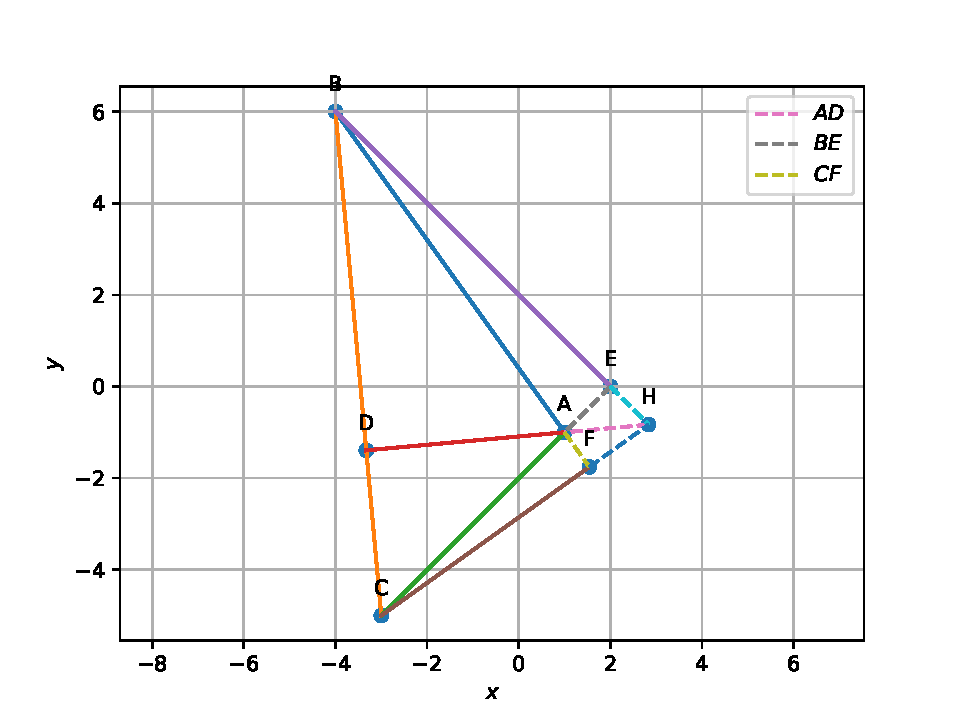
\includegraphics[width=0.75\columnwidth]{figs/triangle/altitude.pdf}
\caption{Altitudes $BE_1$ and $CF_1$ intersect at $\vec{H}$}
\label{fig:m_tri_py}
\end{figure}
\fi
